\begin{appendix}

\section{APPENDIX}
%=========================================
\subsection{Additional Plots}
This section provides additional plots illustrating the performance of the experiments.

Figure~\ref{fig:q_throughput_16} shows the measured throughput,
as images per second, delivered by each system for all queries and databases.
In comparison to figure~\ref{fig:q_throughput_56}, when using fewer concurrent 
clients (nthr = 16), the throughput for VDMS for queries \textit{q4} (\textit{2tag\_or\_resize}), 
\textit{q5} (\textit{2tag\_resize\_geo\_and}), and
\textit{q6} (\textit{2tag\_resize\_geo\_or}) improved by a large margin 
for the 50M and 100M databases. 
In the case of \textit{q4} and \textit{q6}, the throughput for 50M (and 100M for \textit{q4})
increase by a large margin which outperforms both baselines while in figure~\ref{fig:q_throughput_56}
PostgreSQL slightly performed better than VDMS. 
In the case of \textit{q5}, all systems perform a little differently for databases
larger than 5M.  The gaps between the throughput of each system narrows at 10M.  
At a database size of 50M, the performance of the baselines drastically drop
while the throughput of VDMS has a large improvement in comparison.

\begin{figure}[ht]
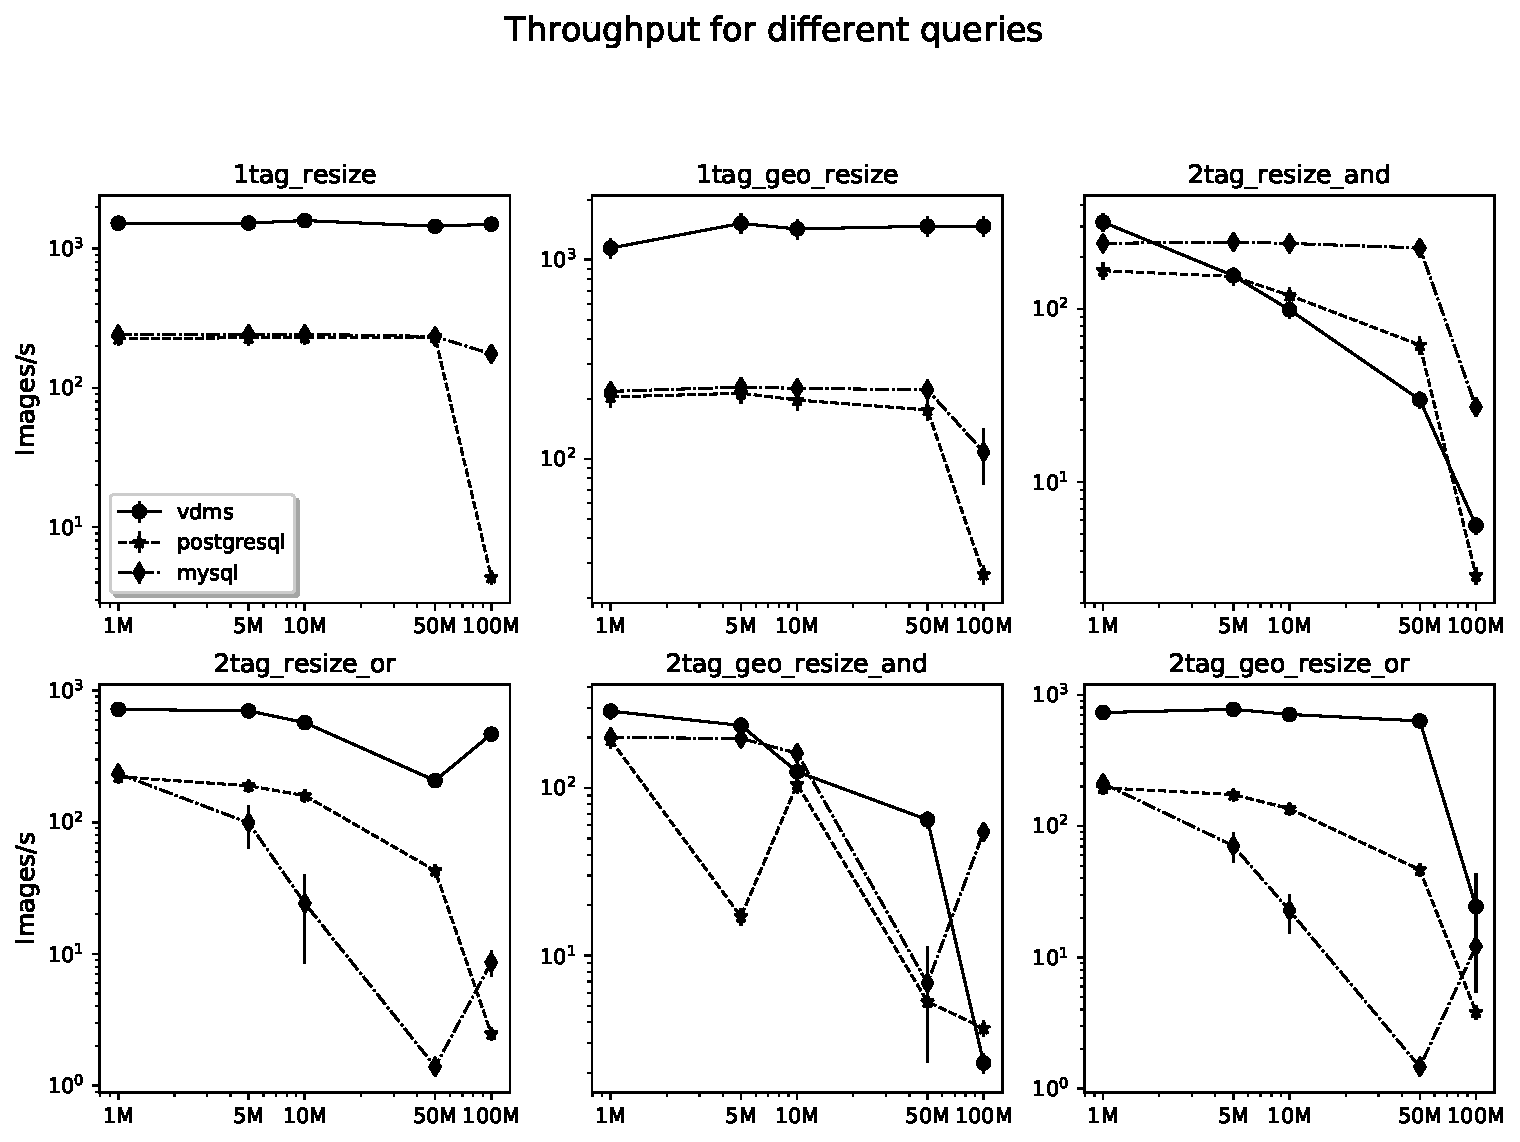
\includegraphics[width=\columnwidth]{figures/plot_th_16_mosaic_results_throughput}
\caption{Throughput Analysis using all queries from our use-case
described in the Experimental Setup Section.
We show queries in different figures for readability reasons.
The experiments show the performance of all systems (VDMS and the two baselines) as the
database size increases.
These queries were run using 16 simultaneous clients (nthr = 16),
and averaged out of 5 runs.}
\label{fig:q_throughput_16}
\end{figure}

Figure~\ref{fig:summary_mysql} summarizes the results
comparing VDMS and MySQL. We see up to 96x speedup (for the case of \textit{q2}),
and an average improvement in throughput of about 31x.
We also see how \textit{q3} and \textit{q5} have poor performances and scalability
as the database size grows same as shown in Figure~\ref{fig:summary_postgresql}.
Considering all other queries (\textit{q1}, \textit{q2}, \textit{q4}, and \textit{q6}), 
VDMS provides at least 3x speedup in throughput.

\begin{figure*}[ht]
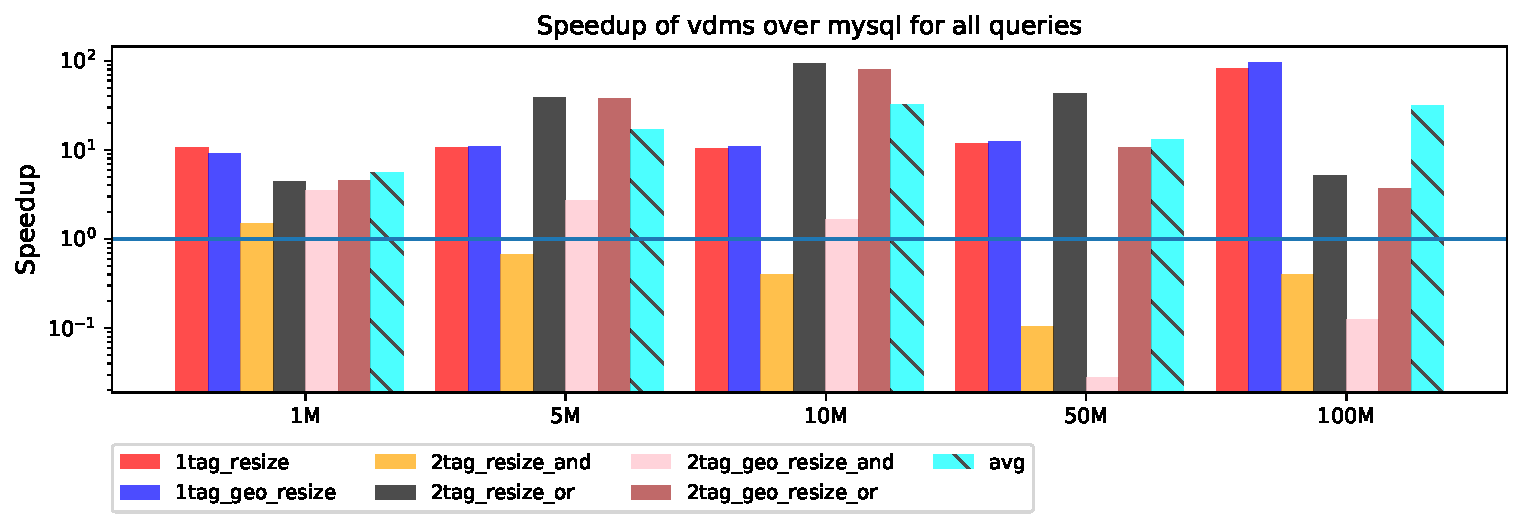
\includegraphics[width=\textwidth]{figures/plot_th_56_query_times_speedup_mysql}
\caption{Summary of performance gains for all queries.
We see up to 96x speedup (\textit{q2}), and an average of about 31x.
More importantly, we see that the speedup grow as the database size increases,
showing that VDMS scales better than the MySQL baseline.}
\label{fig:summary_mysql}
\end{figure*}
%=========================================

\end{appendix}

% \section{APPENDIX - Video Evaluation}
% %=========================================
\subsection{Video Search}
\label{videos}

VDMS provides full support for video storage and operations,
in a similar way it does for images.
This includes support for encoding, decoding, and transcoding of
\textit{mp4}, \textit{avi}, and \textit{mov} containers,
as well as support for \textit{xvid}, \textit{H.263} and \textit{H.264} encoders.
This is supported through the Visual Compute Module that provides an abstraction
layer on top of OpenCV~\cite{opencv} and \textit{libffmpeg}\cite{ffmpeg}.
All operations supported for images in VDMS are also supported at the
video and frame level of the API.
On top of that, there are a number of video-specific operations that
are supported, such as the interval operations,
enabling users to retrieve clips at different
frames-per-second (FPS) versions of the video.

We evaluate the performance and scalability of the video management
capabilities offered by VDMS.
Handling video in a general way is a complex task.
Some of this complexity comes from the existence of a variety of open and
proprietary implementations, different encoding techniques and container
formats, and different parameters of the video itself that are
application-dependent, like frames per second, lossy compression, etc.
When it comes to video, ad-hoc solutions have a large number of parameters that
can be tuned.
Together with that, there is no system that enables transactional
operations over videos files in the way VDMS does.
Because of this, we focus our efforts on understanding variations in the
performance of VDMS and its scalability, rather than comparing
it to a baseline that would not represent a fair
comparison for either of the systems.

\begin{figure*}[ht!]
\centering
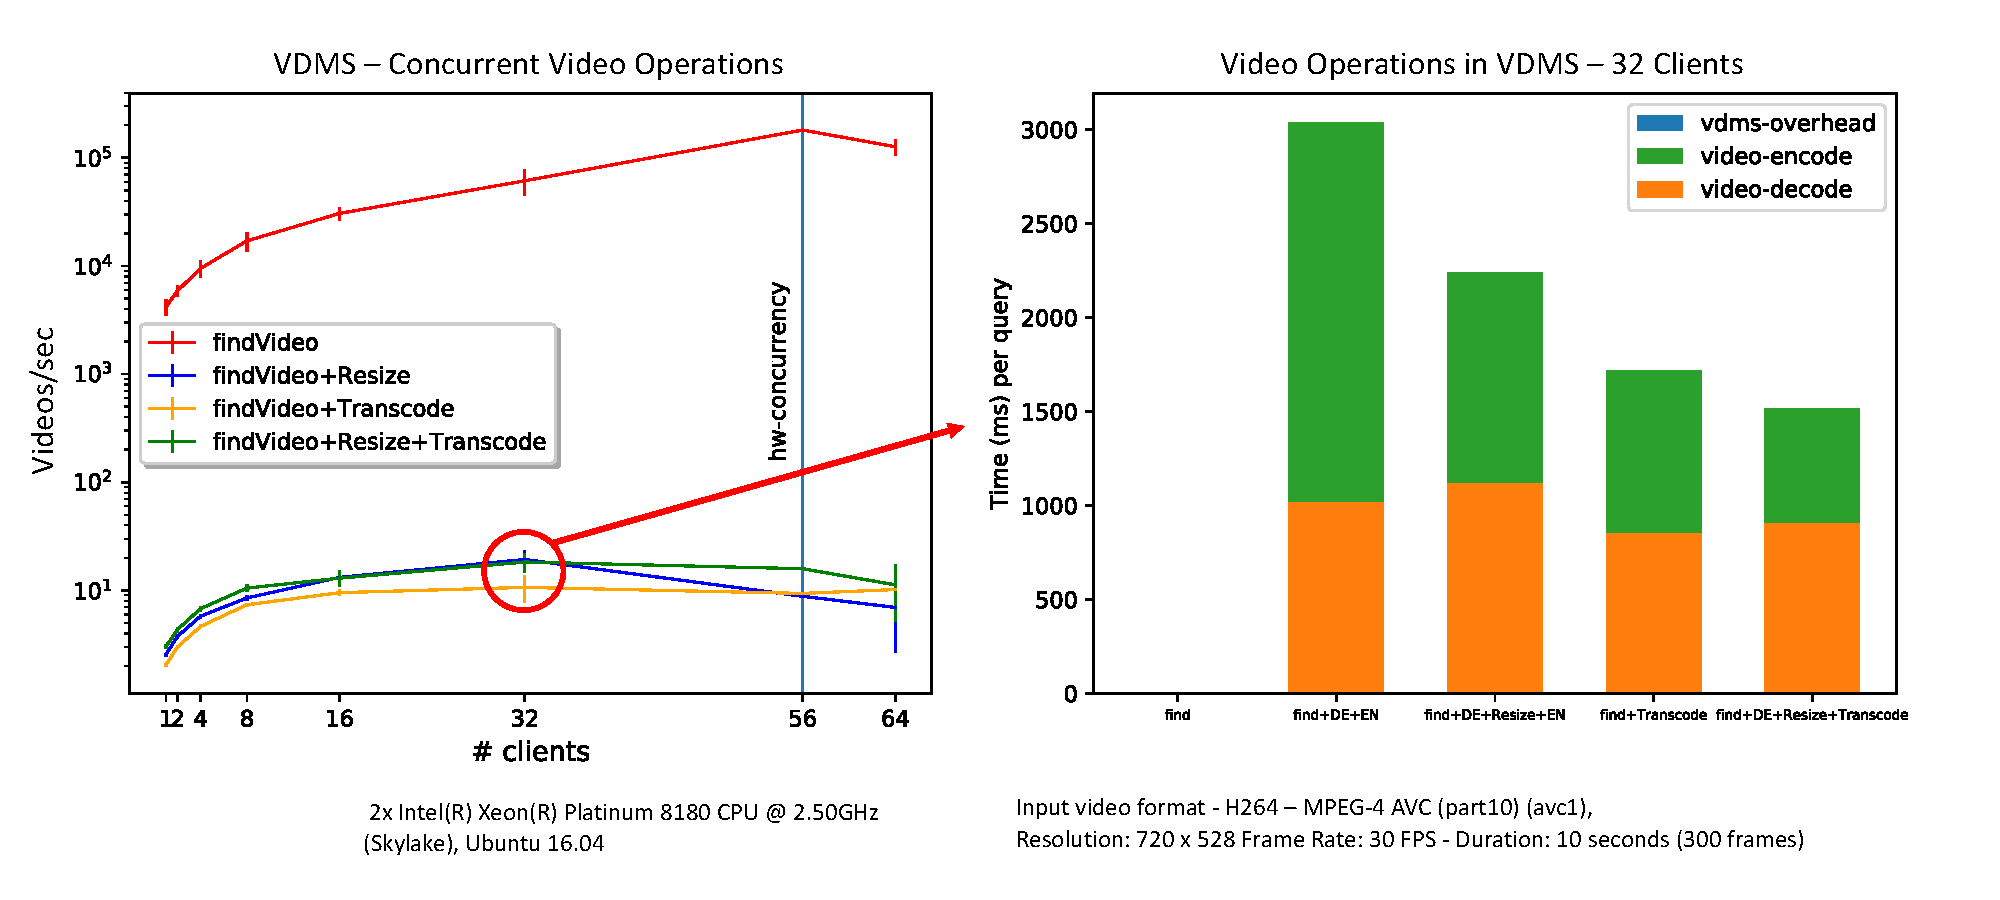
\includegraphics[width=\textwidth]{figures/video_overhead}
\caption{Analysis of video operations. The left figure shows the video throughput (videos per sec) as the number of concurrent clients increase and the right figure breaks down the different components of the
queries using 32 clients.}
\label{fig:video}
\end{figure*}

All this functionality is provided and integrated with the rest of the
metadata API as part of the comprehensive VDMS interface.
This makes it possible for users to interact with metadata and video in
a transactional manner, enabling users to run queries like:
"Retrieve all the videos where there is a \textit{lake} with
probability higher than 0.86, converting all videos to \textit{H.264}
\textit{mp4} of size 224x224".
Appendix shows a sample of how this query would be implemented using the VDMS API
\footnote{https://github.com/IntelLabs/vdms/wiki/FindVideo}.
In particular, this functionality was used internally to select a subset
of videos with the right licenses for a video summarization application.

To the best of our knowledge, there is no solution that can provide
all the functionality mentioned above, behind a single interface
that also allows users to interact with images and metadata.
Implementing a baseline, like we did for images, is significantly more complex
due to the parametrization of video encodings and containers,
as explained at the beginning of this section.
For this reason, we chose to make a study using VDMS in various scenarios,
and analysis of scalability and the impact of having the overhead of VDMS' Request
Server in the overall access time and throughput.

Figure~\ref{fig:video} shows the analysis of different queries aimed
at retrieving a video using the VDMS interface.
We show how VDMS throughput increases when serving
a video object as the number of simultaneous clients increases, as well as the
overhead operations introduced in the overall query execution time.
The figure on the left compares the number of video transaction per second
(i.e., number of videos returned per second) when different operations
are executed as part of the transaction. The upper-bound of this would be
simply returning the video as-is (without running any encoding/decoding or
operation), represented by the red line. This query is the upper-limit because
it essentially translates to reading the video from the file-system and sending
it over a TCP/IP socket, without any other overhead or operations.

\begin{listing}[ht!]
\begin{minted}[frame=single,
               framesep=3mm,
               linenos=true,
               xleftmargin=21pt,
               tabsize=4]{js}
"FindEntity"{
    "class": "autotag",
    "constraints": {
        "name": ["==", "lake"]
    }
    "_ref" : 1
},
"FindVideo":{
    "container": "mp4",
    "codec": "h.264",
    "link": {
        "ref":1,
        "constraints": {
            "prob": [">=", 0.86]
        }
    }
    "operations": [{
        "type": "resize",
        "height": 1080,
        "width":  1920,
    }]
}

\end{minted}
\caption{Sample Query for Video -
The query expresses the following:
Find all videos connected to the autotag \textit{lake}
with probability higher than 0.86, apply a resize operation
to make the video 1920×1080, and convert to "mp4" file,
using H.264 encoding.}
\label{findvideo}
\end{listing}

We also run a set of other queries that involve, showed in Figure~\ref{fig:video}:
(a) running a resize operation on the video and, consequently,
decoding and encoding operations as well (blue line),
(b) transcoding, meaning the use of a different container and encoder
than the one originally used (yellow line), and
(c) both resize and transcoding.
Note that the resize operation (blue and green lines) performs a downsize,
which translates in less data being sent over the wire.
This is specially noticeable when supporting 32 simultaneous clients,
where the system provides more videos per second due to sending less data to
the client, when compared to just transcoding and not resizing (yellow line).
We can see that the system performs best when using all the physical cores,
and this can be attributed to the compute-bound nature of video
encoding, decoding, and processing.

It is important to note an almost 3 orders of magnitude drop in performance
when including operations as part of the query.
We wanted to understand where most of the time was spent on the queries,
and optimize the Request Server and Visual Compute Module
if necessary. For this, we run the experiment shown at
Figure~\ref{fig:video} (right) which breaks down the different components of the
queries. This figure shows that more than 97\% of the query execution is spent
on encoding/decoding operations, which is well-known to be a
compute intensive operation\cite{videosgoogle}.
On the one hand, this result shows that VDMS barely introduces any overhead.
On the other hand, this result means a limit on the opportunities
for optimization for video queries given that biggest time factors
are accounted by encoding/decoding, which is outside the scope of VDMS.
This result was the call to action for one optimization we will include
in future releases of VDMS, which involves using \textit{ffmpeg} C++ API to
limit the number of frames being encoded/decoded when possible.
This functionality will prevent encoding/decoding to happen on all frames
when users only need to retrieve a subset of the frames in the video.

%=========================================

% \clearpage

% \section{APPENDIX - Similarity Search Evaluation}
% 
\begin{figure*}[ht!]
\centering
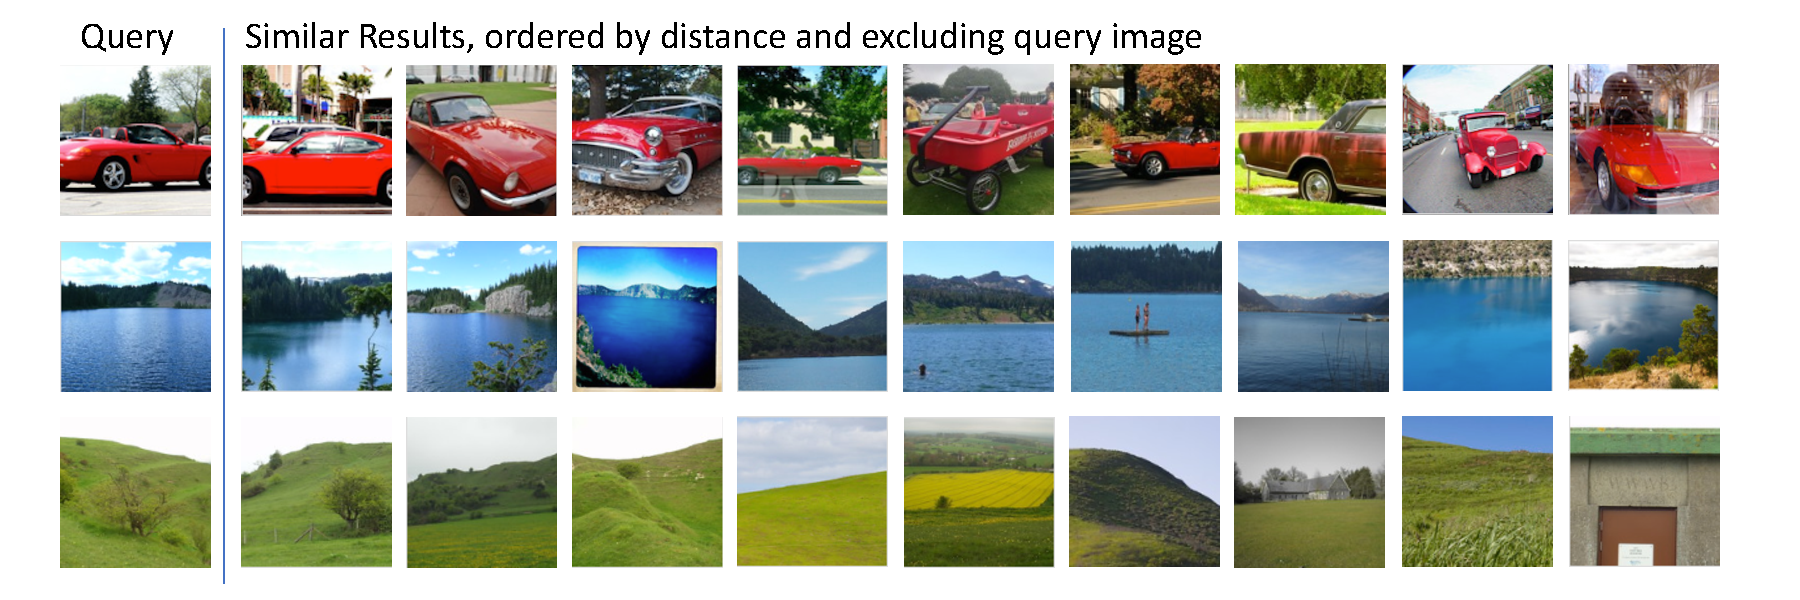
\includegraphics[width=\textwidth]{figures/feature_img_results}
\caption{Sample Results of Similarity Search}
\label{fig:similarity}
\end{figure*}

\subsection{Similarity Search}
\label{features}

Another key differentiating factor of VDMS is that it allows the creation of
indexes for high-dimensional feature vectors and the insertion of
these feature vectors associated with entities, images, and/or videos.
Feature vectors are intermediate results of various machine
learning or computer vision algorithms when run on visual data.
Feature vectors are also known as \textit{descriptors}
or \textit{visual descriptors}. We use these terms interchangeably.
These descriptors can be classified, labeled, and used to build search
indexes. There are many in-memory libraries that are designed for
this task~\cite{flann, faiss}.

% We analyze the behavior of the feature vector functionality in VDMS,
% and an evaluation of the different trade-offs that the systems offers for
% application developers. For this, we implemented an image-search application
% based on \textit{similarity} search.

Using the VDMS API, users can manage feature vector indexes,
query previously inserted elements,
run a k-nearest neighbor search (\textit{knn}), and express relationships
between existing images or descriptors and
the newly inserted descriptors.
By natively supporting descriptors and \textit{knn},
VDMS allows out-of-the-box classification functionalities for many applications
\footnote{https://github.com/\{Not shown during submission\}}.
% \footnote{https://github.com/IntelLabs/vdms/wiki/ClassifyDescriptor}.

For this work, and as part of a comprehensive image search implementation,
we have used 4096-dimensional descriptors extracted from every image
(and first frame of every video) from the YFCC100M dataset
and created a collection of these feature vectors in VDMS to
perform similarity search (i.e., find images that are
\textit{similar} to an query (input) image).
\textit{Similarity} in this particular case is defined as closeness
in a 4096-dimensional space using euclidean distance as the metric.

The process of loading descriptors in VDMS is simple.
First, the user has to create a DescriptorSet, using a single command.
At creation of the DescriptorSet, the dimensionality of the descriptors
is specified, together with the desired indexing method and the desired metric
for computing distances (Euclidean Distance, \textit{L2},
or Inner Product, \textit{IP}).
Once the DescriptorSet is created, descriptors can be inserted to the set.
After the descriptors are inserted, a similarity search can be performed.

Figure~\ref{fig:similarity} shows 3 examples of a query image (on the left),
and images returned as \textit{similar} by VDMS.
The input is a descriptor generated after a query image.
The \textit{query input} descriptor is sent to VDMS as part of the query,
VDMS uses that descriptor to find similar ones,
and retrieves the images associated with those \textit{similar} descriptors.
We show this as an example of the functionality and to depict
how the feature vectors provided by the dataset can be used,
but we also provide an analytical approach to
the trade-off between accuracy and execution time in our system.
It is important to note that the accuracy of the results is entirely tied
to the quality of the descriptors chosen by the applications.
The quality of the similarity result will be tied to the quality
of the descriptor extraction that the application is using.

\begin{figure*}[ht]
\centering
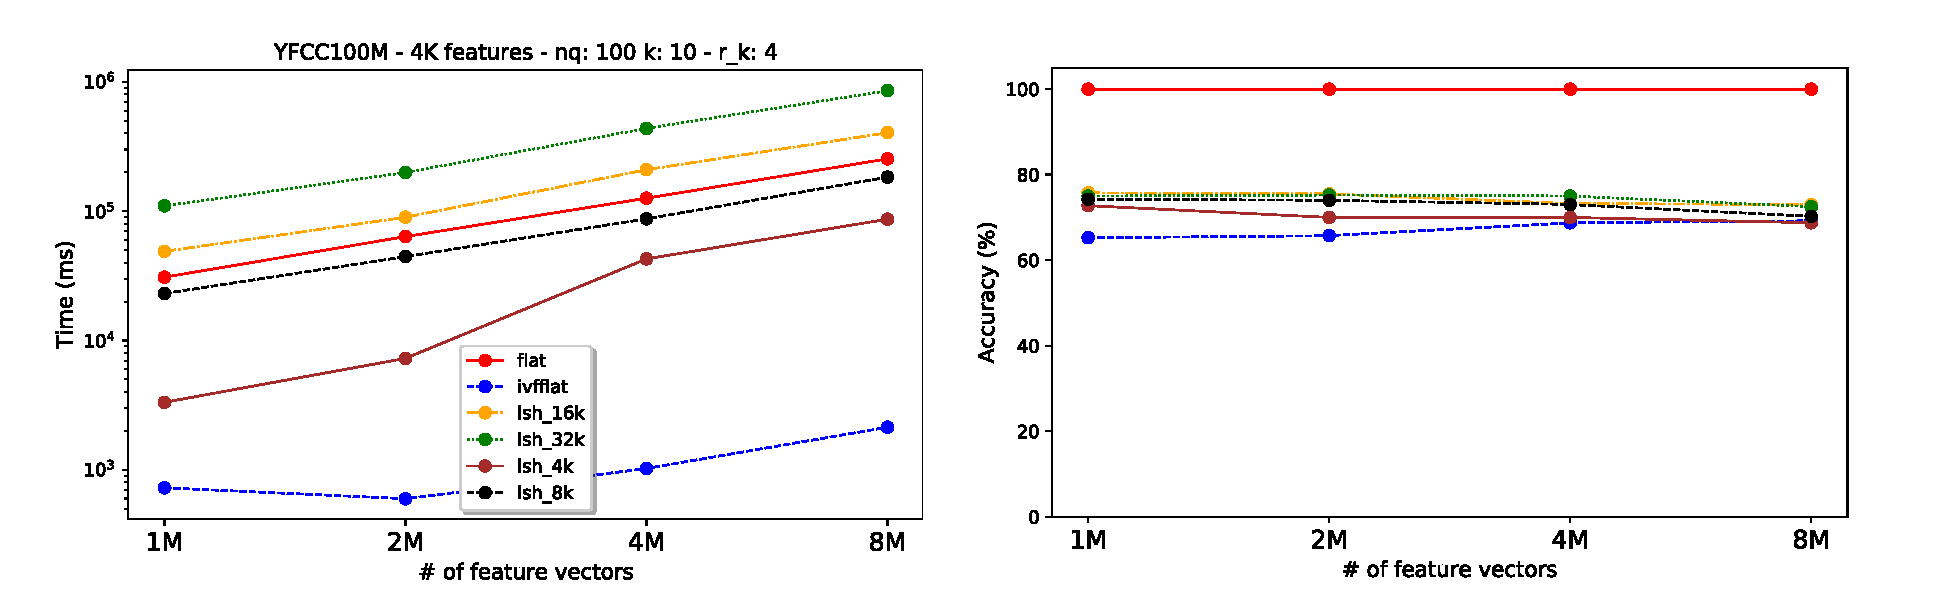
\includegraphics[width=\textwidth]{figures/features_alternatives}
\caption{Feature Vector Evaluation: Trade-off between query execution speed
and accuracy of the results, using ground-truth data for computing accuracy.
For this evaluation, we query the 10 closest neighbors (k = 10), and compute
accuracy using recall at 4 (r\_k = 4) (i.e. percentage of the top 4 ground-truth
results that is present within the top 10 computed neighbors).
We average the query execution time and accuracy for 100 queries (nq = 100).}
\label{fig:features_eval}
\end{figure*}

\begin{figure*}[ht]
\centering
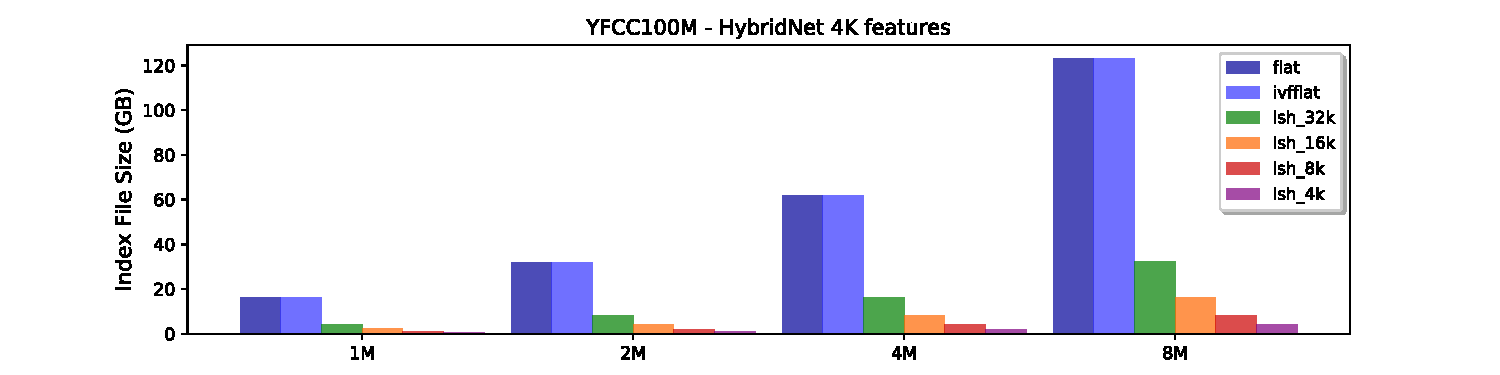
\includegraphics[width=\textwidth]{figures/features_disksize}
\caption{Feature Collection Size in Disk}
\label{fig:features_size_does_matter}
\end{figure*}

As mentioned before, VDMS provides different levels of customization of the
indexes created for a descriptor set, that includes the indexing techniques
and the metric for similarity.
These different indexing techniques come with different trade-offs in terms
of speed of search and accuracy of the computation.
VDMS aims to provide functionality that is agnostics to application-specific
techniques, enabling features that are generic to visual data processing
applications.
Figure~\ref{fig:features_eval} shows an analysis at the different indexing
techniques provided by VDMS and its trades-off between accuracy and query
execution speed, for a single threaded client.
For this evaluation, we query the 10 closest neighbors (k = 10), and compute
accuracy using recall at 4 (r\_k = 4) (i.e. percentage of the top 4 ground-truth
results that is present within the top 10 computed neighbors).
We average the query execution time and accuracy for 100 queries (nq = 100).
The \textit{flat} index (red line) implements exact search and
represents ground-truth, which explain why the
accuracy is always 100\% in the plot on the right.
The other indexes implement \textit{approximate search},
which trades-off between accuracy and speed of search~\cite{flann, faiss}.
We have also tried the \textit{ivfflat} index (inverted file index), as well as
\textit{LSH}-based indexes using a different number of bits per descriptor
\footnote{https://github.com/facebookresearch/faiss/wiki/Faiss-indexes}.
Results show how \textit{ivfflat} is the fastest option but it comes with a trade-off
of about 30\% loss in accuracy, while simple brute-force search
is among the slowest options at the expenses of 100\% accuracy,
meaning exact search.

Another important trade-off to be made is with respect to space efficiency:
The DescriptorSet can grow very large and expensive to load and manage.
In this particular case, 4096-dimensional descriptors for 100M elements
translates into 1TB of data, only in raw floating-point data alone
(without accounting for any metadata or indexes associated with it).
This component is very important for the overall analysis on which
index structure to use because a large set of descriptors may not fit in memory
and thus cause a pressure on the IO system while retrieving descriptors
for computing distance.
This can severely impact the overall query execution time.
When the DescriptorSet grows significantly large,
it may be worth trading off accuracy for speed and space.
Figure~\ref{fig:features_size_does_matter} shows the different indexes and
their size in disk. These indexes already contain all the descriptors (or
a quantized version of them in the case of LSH~\cite{lsh}),
and can be loaded in memory directly when it fits.
Note how, because of quantization of the descriptors, \textit{LSH} provides a
significantly lower space foot print, which can be a great option for
large collections of descriptors when accuracy is not a main factor.
It is not uncommon to sacrifice accuracy as images and videos are captured
using a noise sensor (i.e., the camera), and an approximate search
in many cases can provide the necessary accuracy for applications
to achieve their goals.


% \section{APPENDIX - API Samples}

% \begin{appendix}

% \begin{listing}[ht!]
% \begin{minted}[frame=single,
%               framesep=3mm,
%               linenos=true,
%               xleftmargin=21pt,
%               tabsize=4]{js}
% "FindEntity"{     
%     "class": "autotag",
%     "constraints": { 
%         "name": ["==", "alligator"]
%     }
%     "_ref" : 1
% },
% "FindImage":{
%     "format": "png",
%     "link": {
%         "ref":1,
%         "constraints": {
%             "prob": [">=", 0.66]
%         }
%     }
%     "operations": [{
%         "type": "resize",
%         "height": 224,
%         "width":  224,
%     }]
% }

% \end{minted}
% \caption{Sample Query for Images - 
% The query expresses the following: 
% Find all the images connected to the autotag \textit{alligator} 
% with probability higher than 0.66, apply a resize operation
% to make the images 224x224, and convert to "png".} 
% \label{findimage}
% \end{listing}

% \begin{listing}[t!]
% \begin{minted}[frame=single,
%               framesep=3mm,
%               linenos=true,
%               xleftmargin=21pt,
%               tabsize=4]{js}
% "FindEntity"{     
%     "class": "autotag",
%     "constraints": { 
%         "name": ["==", "alligator"]
%     }
%     "_ref" : 1
% },
% "FindImage":{
%     "format": "png",
%     "link": {
%         "ref":1,
%         "constraints": {
%             "prob": [">=", 0.66]
%         }
%     }, 
%     "constraints": {
%         "latitude": [">=", 36.23433, 
%                      "<=", 38.23433]
%         "longitude":[">=", -114.80666, 
%                      "<=", -116.80666]
%     },
%     "operations": [{
%         "type": "resize",
%         "height": 224,
%         "width":  224,
%     }, {
%         "type": "rotate",
%         "angle": 45.34
%     }]
% }

% \end{minted}
% \caption{Sample Query for Images - 
% The query expresses the following: 
% Find all the images connected to the autotag \textit{alligator} 
% with probability higher than 0.66, 
% filter by latitude and longitude within 1 degree, 
% apply a resize operation to make the images 224x224
% and rotate the image 45.34 degrees, 
% and return the images as "png" files.} 
% \label{findimagegeo}
% \end{listing}

% \end{appendix}
